%%%%%%%%%%%%%%%%%%%%%%%%%%%%%%%%%%%%%%%%%
% Beamer Presentation
% LaTeX Template
% Version 1.0 (10/11/12)
%
% This template has been downloaded from:
% http://www.LaTeXTemplates.com
%
% License:
% CC BY-NC-SA 3.0 (http://creativecommons.org/licenses/by-nc-sa/3.0/)
%
%%%%%%%%%%%%%%%%%%%%%%%%%%%%%%%%%%%%%%%%%

%----------------------------------------------------------------------------------------
% PACKAGES AND THEMES
%----------------------------------------------------------------------------------------

\documentclass{beamer}

\mode<presentation> {

% The Beamer class comes with a number of default slide themes
% which change the colors and layouts of slides. Below this is a list
% of all the themes, uncomment each in turn to see what they look like.

% \usetheme{default}
% \usetheme{AnnArbor}
% \usetheme{Antibes}
%\usetheme{Bergen}
%\usetheme{Berkeley}
%\usetheme{Berlin}
%\usetheme{Boadilla}
%\usetheme{CambridgeUS}
%\usetheme{Copenhagen}
%\usetheme{Darmstadt}
%\usetheme{Dresden}
%\usetheme{Frankfurt}
%\usetheme{Goettingen}
%\usetheme{Hannover}
%\usetheme{Ilmenau}
%\usetheme{JuanLesPins}
% \usetheme{Luebeck}
\usetheme{Madrid}
% \usetheme{Malmoe}
%\usetheme{Marburg}
%\usetheme{Montpellier}
%\usetheme{PaloAlto}
%\usetheme{Pittsburgh}
%\usetheme{Rochester}
% \usetheme{Singapore}
%\usetheme{Szeged}
%\usetheme{Warsaw}

% As well as themes, the Beamer class has a number of color themes
% for any slide theme. Uncomment each of these in turn to see how it
% changes the colors of your current slide theme.

%\usecolortheme{albatross}
%\usecolortheme{beaver}
% \usecolortheme{beetle}
%\usecolortheme{crane}
%\usecolortheme{dolphin}
%\usecolortheme{dove}
% \usecolortheme{fly}
%\usecolortheme{lily}
%\usecolortheme{orchid}
%\usecolortheme{rose}
%\usecolortheme{seagull}
% \usecolortheme{seahorse}
%\usecolortheme{whale}
%\usecolortheme{wolverine}

%\setbeamertemplate{footline} % To remove the footer line in all slides uncomment this line
%\setbeamertemplate{footline}[page number] % To replace the footer line in all slides with a simple slide count uncomment this line

%\setbeamertemplate{navigation symbols}{} % To remove the navigation symbols from the bottom of all slides uncomment this line
}

\usepackage{graphicx} % Allows including images
\usepackage{booktabs} % Allows the use of \toprule, \midrule and \bottomrule in tables
\usepackage{subcaption}
\usepackage{indentfirst}
\setbeamertemplate{caption}[numbered]

%----------------------------------------------------------------------------------------
% TITLE PAGE
%----------------------------------------------------------------------------------------

\title[Visual Analytics Towards Big Data]{Visual Analytics Towards Big Data} % The short title appears at the bottom of every slide, the full title is only on the title page

\author{Shen Tianma, Yuan Jihong, Liu Yehui \texorpdfstring{\\ Chen Yaru, Jiang Haishu, Shi Bin}{} } % Your name
\institute[USST] % Your institution as it will appear on the bottom of every slide, may be shorthand to save space
{
University of Shanghai for Science and Technology \\ % Your institution for the title page
\medskip
\textit{} % Your email address 
}
\date{\today} % Date, can be changed to a custom date

\begin{document}

\begin{frame}
\titlepage % Print the title page as the first slide
\end{frame}

\begin{frame}
\frametitle{Overview} % Table of contents slide, comment this block out to remove it
\tableofcontents % Throughout your presentation, if you choose to use \section{} and \subsection{} commands, these will automatically be printed on this slide as an overview of your presentation
\end{frame}

%----------------------------------------------------------------------------------------
% PRESENTATION SLIDES
%----------------------------------------------------------------------------------------

\section{Information Visualization}

\subsection{Introduction of Information Visualization}
\begin{frame}
  \frametitle{Introduction of Information Visualization}
  \qquad Information visualization or information visualisation is the study of (interactive) visual representations of abstract data to reinforce human cognition. The abstract data include both numerical and non-numerical data, such as text and geographic information.\\

  \begin{itemize}
    \item visual representations of abstract data 
    \item different from scientific visualization
    \item emergence from research in human-computer interaction, computer science, graphics, visual design, psychology, and business methods
  \end{itemize}

\end{frame}


\subsection{Specific methods and techniques}

\begin{frame}
  \frametitle{Specific methods and techniques}

  \begin{itemize}
    \item Cartogram
    \item Cladogram (phylogeny)
    \item Concept Mapping
    \item Dendrogram (classification)
    \item Information visualization reference model
    \item Graph drawing
    \item Heatmap
    \item HyperbolicTree
    \item Multidimensional scaling
    \item Parallel coordinates
    \item Problem solving environment
    \item Treemapping
  \end{itemize}
\end{frame}

\begin{frame}
  \frametitle{Heatmap}
  \begin{figure}
    \begin{center}
      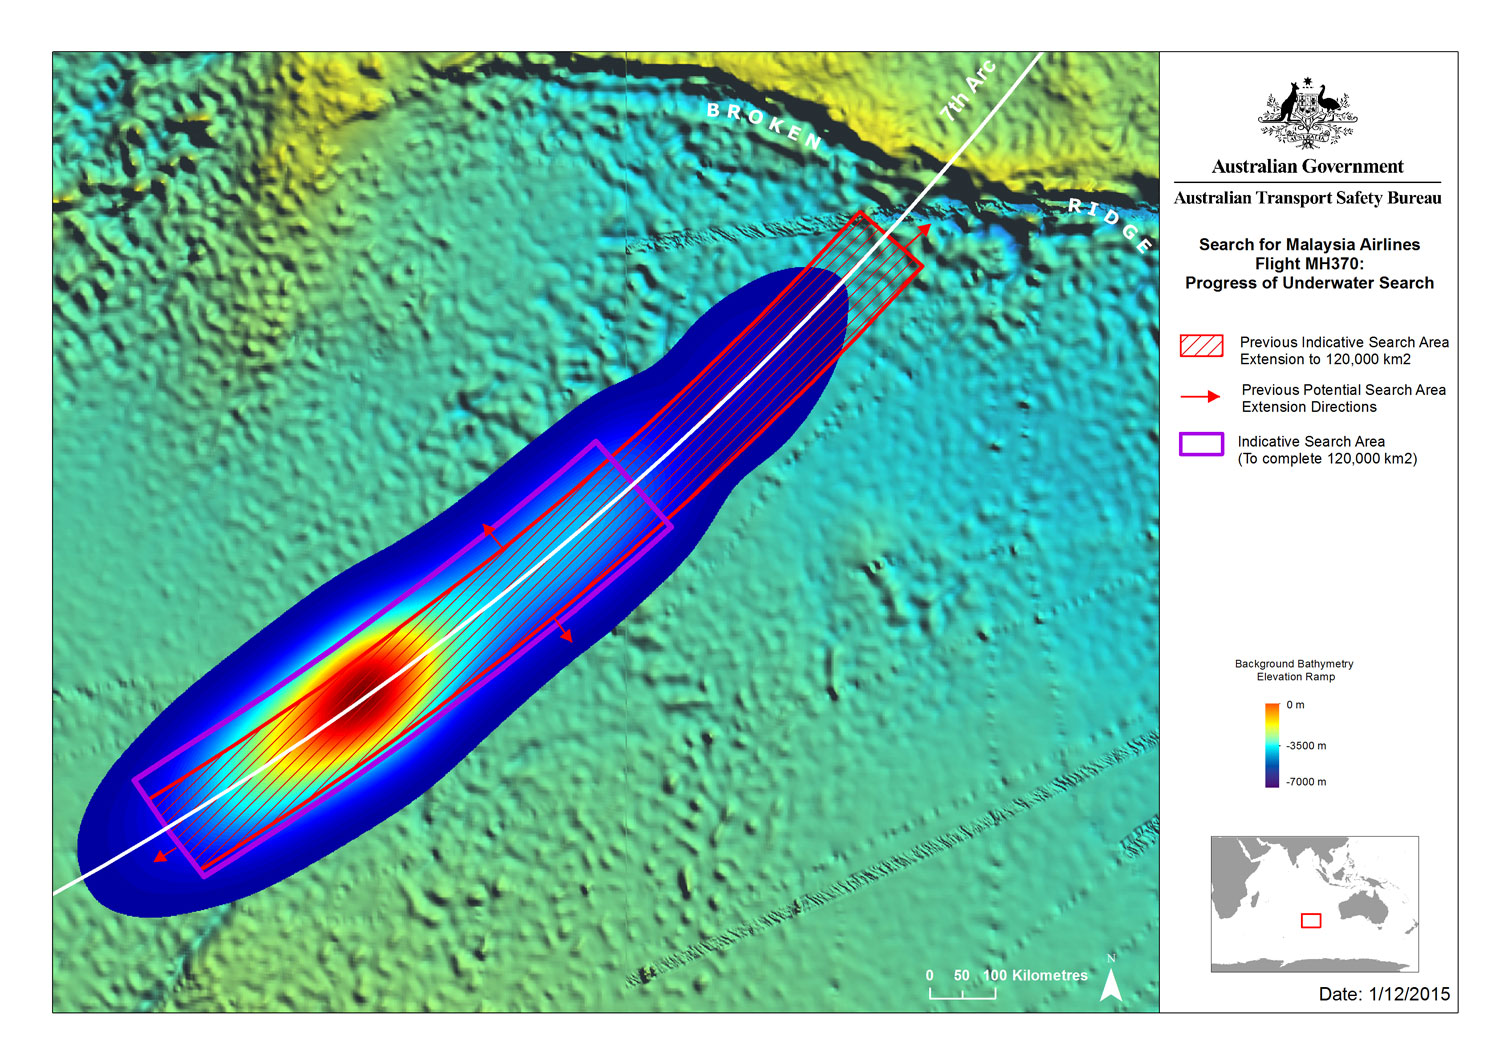
\includegraphics[width=0.8\linewidth]{images//heat.jpg}
      \caption{MH370 location probability heat map}
      \label{Fig:1}
    \end{center}
    % \vspace{-0.1em}
  \end{figure}
\end{frame}

\begin{frame}
  \frametitle{Heatmap - color schemes}
  \qquad Rainbow colormaps are often used, as humans can perceive more shades of color than they can of gray. However, this is discouraged by many in the scientific community, for the following reasons:  
  \footnote{\tiny{Borland;  Russell (2007). "Rainbow Color Map (Still) Considered Harmful". IEEE Computer Graphics and Applications.}}

  \begin{itemize}
    \item The colors lack the natural perceptual
      \footnote{\tiny{How NOT to Lie with Visualization – Bernice E. Rogowitz and Lloyd A. Treinish – IBM Thomas J. Watson Research Center.}}

    \item Common colormaps have uncontrolled changes
      \footnote{\tiny{Harrower, Mark; Brewer, Cynthia A. (2003). "ColorBrewer.org: An Online Tool for Selecting Colour Schemes for Maps".}}

    \item Not actually present
      \footnote{\tiny{Green, D. A. (2011). "A colour scheme for the display of astronomical intensity images".}}

  \end{itemize}

\end{frame}

\begin{frame}
  \frametitle{Multidimensional scaling}
  \qquad Multidimensional scaling (MDS) is a means of visualizing the level of similarity of individual cases of a dataset. It refers to a set of related ordination techniques used in information visualization, in particular to display the information contained in a distance matrix. It is a form of non-linear dimensionality reduction.\\
  \qquad General forms of loss functions called Stress in distance MDS and Strain in classical MDS. The strain is given by:
  \footnote{\tiny{Borg,, I.; Groenen, P. (2005). Modern Multidimensional Scaling: theory and applications (2nd ed.). }}

  \begin{eqnarray}
    \min _{x_{1},x_{2}\ldots x_{n}}\left( \sum _{i < j}\left( \left\| x_{i}-x_{j}\right\| -d_{ij}\right) ^{2}\right) ^{\dfrac {1}{2}}
  \end{eqnarray}


\end{frame}

\section{Human-computer Interaction}

\subsection{Introduction of Human-computer Interaction}

\begin{frame}
  \frametitle{Introduction of Human-computer Interaction}
  \qquad Human–computer interaction (commonly referred to as HCI) researches the design and use of computer technology, focused on the interfaces between people (users) and computers. \\
  \qquad Much of the research in the field of human-computer interaction takes an interest in:
  \begin{itemize}
    \item Methods for optimizing a design for a desired property.
    \item Methods for evaluating and comparing interfaces.
    \item Methods for studying human computer use more broadly.
    \item Conceptual frameworks for the design of computer interfaces.
    \item Perspectives that critically reflect upon the values.

  \end{itemize}
\end{frame}

\subsection{Topics in HCI}
\begin{frame}
  \frametitle{Topics in HCI}
  \begin{itemize}
    \item User customization.
    \item Embedded computation.
    \item Augmented reality.
    \item Knowledge-driven human-computer interaction.

  \end{itemize}
\end{frame}

\begin{frame}
  \frametitle{Augmented reality}
  AR - Augmented Reality
  \begin{figure}
    \begin{center}
      \includegraphics[width=0.7\linewidth]{images//AR.jpeg}
      \caption{AR - Augmented Reality}
      \label{Fig:4}
    \end{center}
    % \vspace{-0.1em}
  \end{figure}
\end{frame}

\begin{frame}
  \frametitle{Augmented reality}
  VR - Virtual Reality
  \begin{figure}
    \begin{center}
      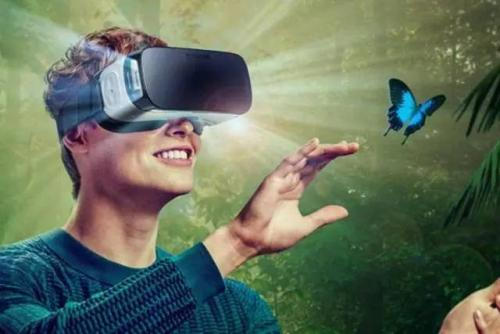
\includegraphics[width=0.7\linewidth]{images//vr.jpg}
      \caption{VR - Virtual Reality}
      \label{Fig:5}
    \end{center}
    % \vspace{-0.1em}
  \end{figure}
\end{frame}

\begin{frame}
  \frametitle{Augmented reality}
  HUD - Head Up Display
  \begin{figure}
    \begin{center}
      \includegraphics[width=0.7\linewidth]{images//hud.jpeg}
      \caption{HUD - Head Up Display}
      \label{Fig:6}
    \end{center}
    % \vspace{-0.1em}
  \end{figure}
\end{frame}





\section{Visual Analytics}

\subsection{Introduction of Visual Analytics}

\begin{frame}
  \frametitle{Introduction of Visual Analytics}
  \qquad Visual analytics is an outgrowth of the fields of information visualization and scientific visualization that focuses on analytical reasoning facilitated by interactive visual interfaces. Visual analytics integrates new computational and theory-based tools with innovative interactive techniques and visual representations to enable human-information discourse.

\end{frame}

\subsection{Implement of Visual Analytics}

\begin{frame}
  \frametitle{Tableau}
  \begin{figure}
    \begin{center}
      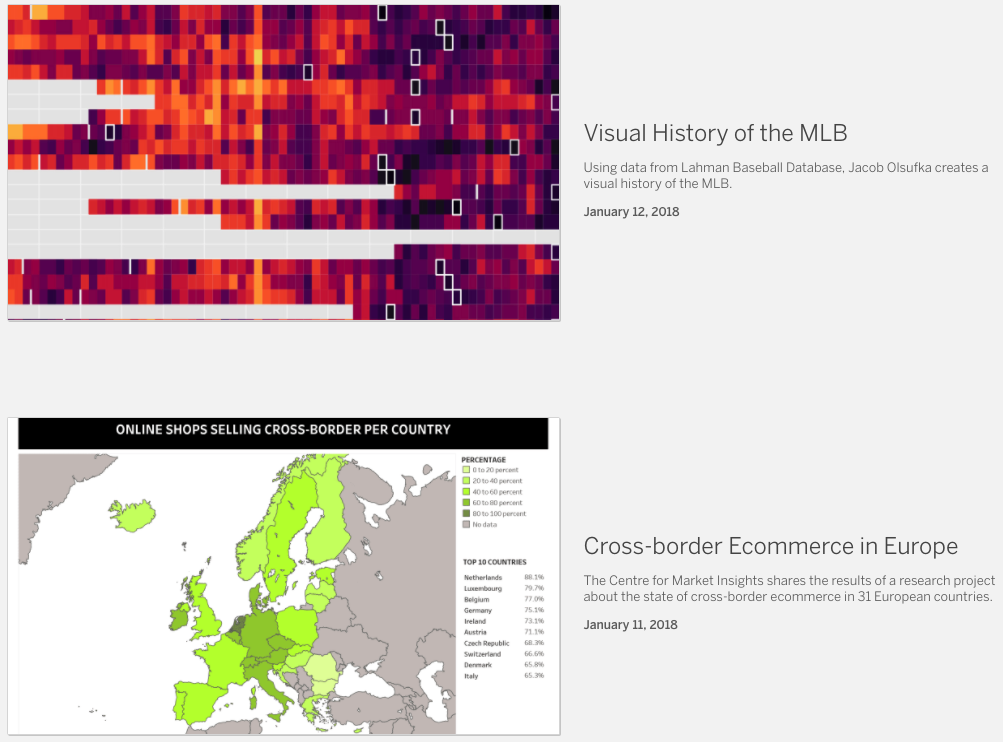
\includegraphics[width=0.7\linewidth]{images//tab.png}
      \caption{Tableau : https://public.tableau.com/zh-cn/s/gallery}
      \label{Fig:7}
    \end{center}
    % \vspace{-0.1em}
  \end{figure}

\end{frame}

\begin{frame}
  \frametitle{Matlab}
  \begin{figure}
    \begin{center}
      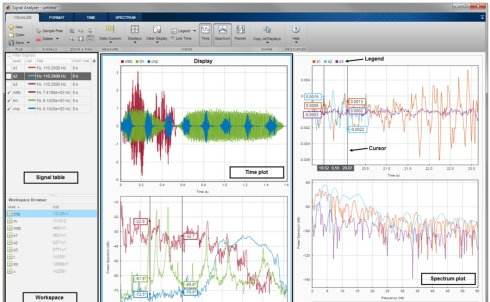
\includegraphics[width=0.7\linewidth]{images//matlab.jpeg}
      \caption{Matlab : https://cn.mathworks.com/}
      \label{Fig:8}
    \end{center}
    % \vspace{-0.1em}
  \end{figure}

\end{frame}

\end{document} 